\section{Proces pomiarowy i~budowa zbioru danych}

\section{Analiza zebranych obrazów termowizyjnych}

\subsection{Prezentacja przykładowej serii pomiarowej}

\subsection{Przetwarzanie danych wizyjnych}

\subsection{Poprawa jakości obrazu}

\subsection{Automatyczny odczyt zakresu pomiarowego temperatur z~obrazu}
Jak wspomniano w~sekcji \ref{subsec:camsoft} jednym z~kluczowych czynników
decydujących o~wyglądzie obrazów pochodzących z~kamery jest zakres temperatur
mapowany na kolory w~obrazie.
Niestety aplikacja FLIR Tools nie pozwala na eksport zakresu temperatur wraz
ze zdjęciami w~formie liczbowej.
W~czasie zapisu zdjęć oprogramowanie dodaje na nich interfejs z~aktywną skalą
pomiarową, jednak jest on graficznie naniesiony na obraz.
Aby ułatwić w przyszłości pracę z~materiałami z~kamery opracowano dodatkowo
mechanizm ekstrakcji zakresu temperatur z~zdjęć pochodzących z kamery.

W~celu konstrukcji funkcji odczytu wartości liczbowych z~obrazu posłużono
się gotową siecią neuronową zaprojektowaną do detekcji tekstu na zdjęciach.
Zdecydowano się na użycie popularnej biblioteki \emph{Pytesseract}.
Aby poprawnie odczytać wartości z~obrazu najpierw przycięto je tak by w~kadrze
znajdowała się tylko odczytywana liczba.
Ponieważ przy eksporcie zdjęć program FLIR Tools nakłada interfejs na zdjęcia
w~identyczny sposób, kadrowanie obrazu jest takie same dla każdej próbki
pomiarowej.
Wycięte kadry są bardzo małej rozdzielczości, aby ułatwić sieci rozpoznawanie
liczb zdecydowano się przeskalować je w~górę.
W~czasie skalowania włączono mechanizm anty aliasingu aby wyrównać krawędzie
cyfr.
Ponieważ używana sieć uznaje za tło kolor biały oraz poszukuje liczb w~kolorze
czarnym barwy na zdjęciu odwrócono.
Następnie obraz poddano binaryzacji metodą \emph{otsu}.
Jest to popularna i~wydajna metoda binaryzacji, jej efektywność jest
maksymalna kiedy ilość pikseli tła oraz pierwszego planu jest zbliżona,
dlatego poprawne kadrowanie liczb sprzyja jakości ich binaryzacji\cite{sezgin}.
Na rysunku \ref{fig:temp_bounds} przedstawiono kolejne etapy przygotowania
obrazu do rozpoznania liczb.
Implementację opisanego mechanizmu odczytywania zakresu temperatur ze zdjęć
przedstawiono na listingu \ref{lst:temp_bounds}.

\begin{figure}[h]
	\centering
	\begin{subfigure}[h]{0.45\textwidth}
		\centering
		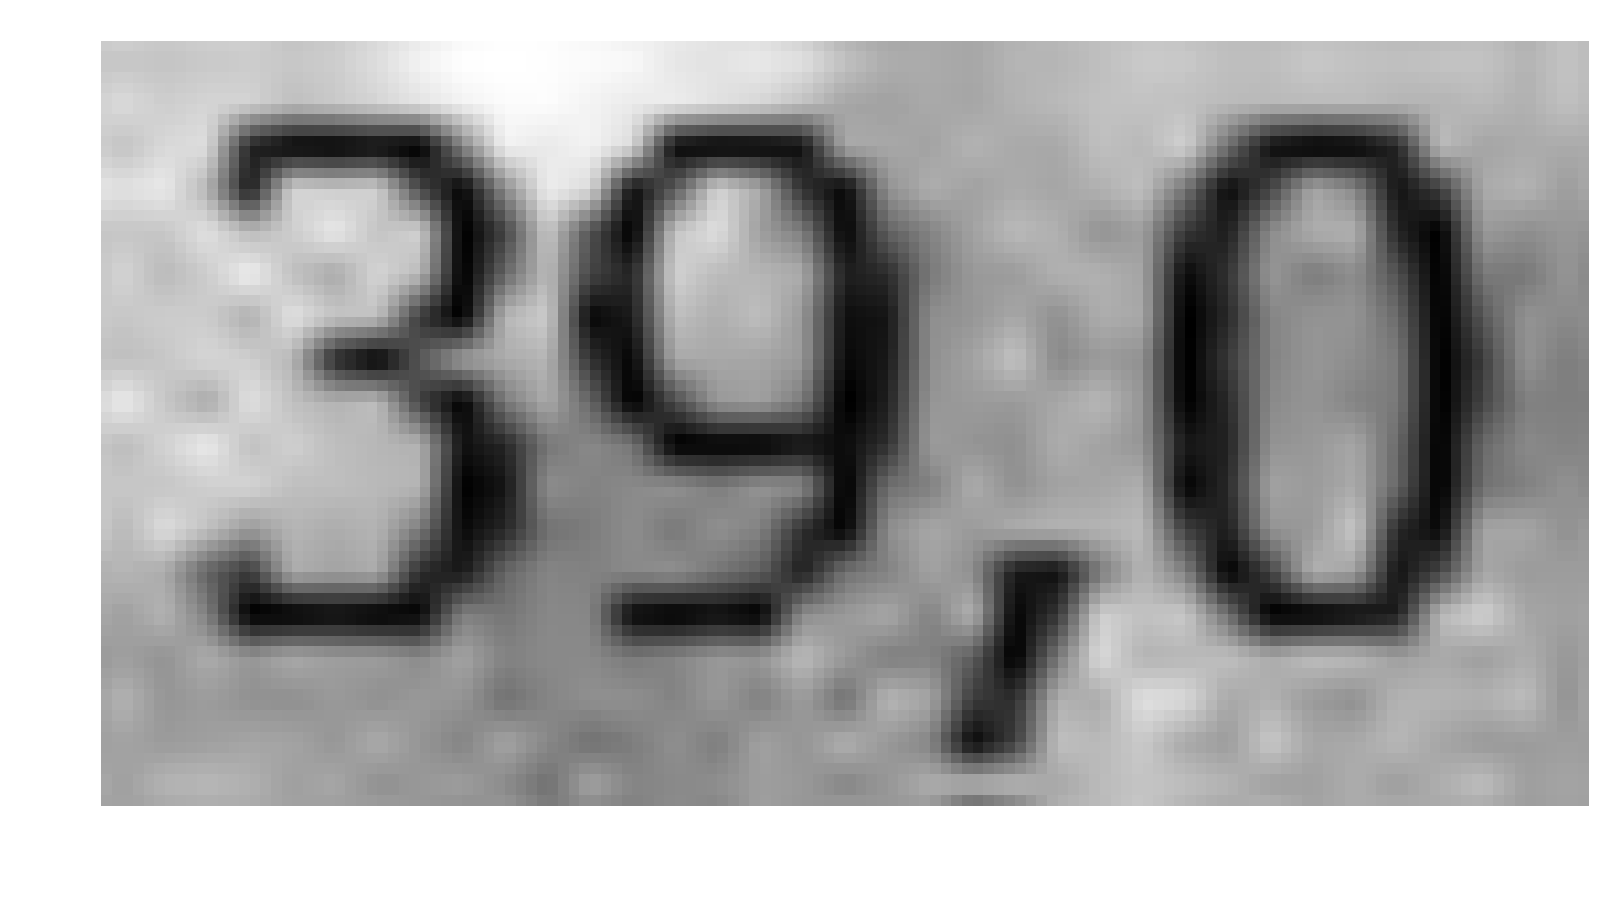
\includegraphics[width=\textwidth]{temp_bounds_scale}
		\caption{Przeskalowany kadr z~liczbą}
		\label{fig:temp_bounds_scale}
	\end{subfigure}
	\quad
	\begin{subfigure}[h]{0.45\textwidth}
		\centering
		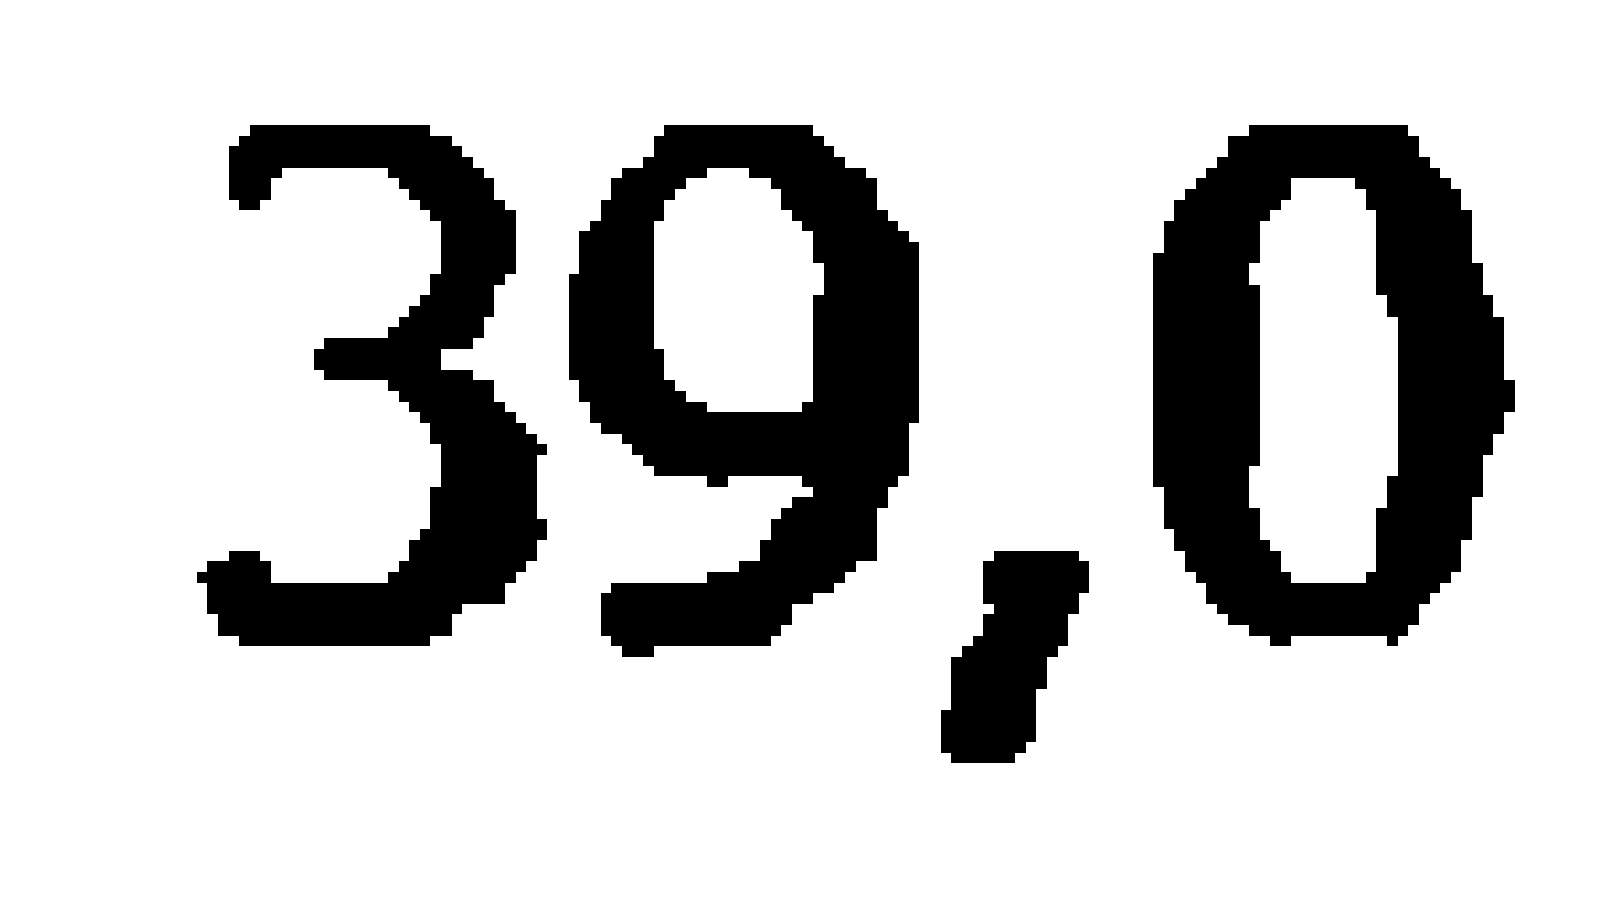
\includegraphics[width=\textwidth]{temp_bounds_bin}
		\caption{Kadr z~liczbą po binaryzacji}
		\label{fig:temp_bounds_bin}
	\end{subfigure}
	
	\caption{Przygotowanie zakresu temperatur do odczytu przez sieć neuronową}
	\label{fig:temp_bounds}
\end{figure}

\begin{listing}[h]
\begin{minted}{python}
def get_temperature_bounds(img, bounds=(((6, 24), (283, 318)),
                                       ((219, 236), (283, 318)))):
    '''Extract temperature values from FLIR UI on image.'''
    img = invert(img)
    temp_txt = []
    for bound in bounds:
        bound_img = img[slice(*bound[0]), slice(*bound[1])]
        bound_img = rescale(bound_img, 4, anti_aliasing=True)
        thr = threshold_otsu(bound_img)
        img_txt = bound_img > thr
        img_txt = Image.fromarray(img_txt)
        temp = pytesseract.image_to_string(img_txt, config='digits')
        if temp is not '': 
            temp = float(temp)
        else:
            temp = 0
        temp_txt.append(temp)
    return temp_txt
\end{minted}
\caption{Funkcja języka Python do odczytywania zakresu temperatur ze zdjęć
         z~kamery}
\label{lst:temp_bounds}
\end{listing}


\section{Poszukiwanie zależności użytecznych w~klasyfikacji}

\subsection{Rozważane możliwości użycia cech obrazu w~klasyfikacji}

\subsection{Wybór algorytmu detekcji ziaren}

\subsection{Algorytm śledzenia ziaren w~serii zdjęć}

\subsection{Wizualizacja zebranych cech i~ocena ich użyteczności}
